\subsection{Literature Review}

\begin{figure}[!htbp]
	\centering
		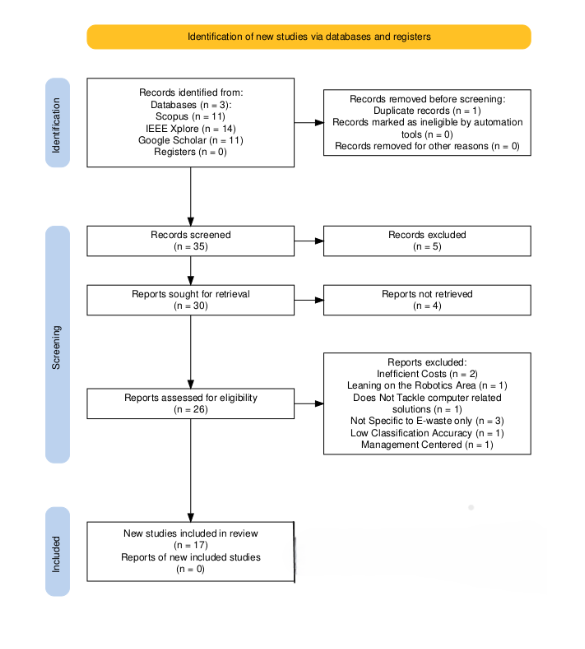
\includegraphics[width=0.5\textwidth]{PRISMA_Diagram.png}
	\caption{PRISMA Diagram}
	\label{fig:Literature Review} %?? ano bang label to
\end{figure}

The PRISMA diagram illustrates the 	systematic process that was done for selecting studies for review through screening and identification. The search identified 35 records from Scopus and IEEE Xplore along with Google Scholar though one duplicate record was excluded from the total. The evaluation of 35 records resulted in five exclusions which reduced the number of reports needed for retrieval to 30. The assessment of eligibility was reduced to 26 reports after four reports were unobtainable. The review process initiated with 35 reports but nine studies were eliminated because of respective reasons that included inefficient cost structure (2) and robot-centered research (1) while a third was considered irrelevant for computer product solutions (1). The evaluation also eliminated three studies because they lacked precision in e-waste coverage and one because of insufficient classification accuracy as well as one because it focused on management practices. The final review included 17 studies only while no new studies were reported. The methodology included specific criteria to choose only research that met the standards of relevance and quality.

\section{Existing Work}
Many studies have examined different waste management strategies, with an emphasis on the collection and disposal of e-waste. In the study of Nowakowski and Pamuła (2020), the researchers explored the use of convolutional neural networks (CNN) and Faster R-CNN for recognizing different objects, focusing specifically on improving e-waste collection strategies. While their deep learning-based system achieved an impressive classification performance of 96.7\% with CNN2, it faced challenges due to the small dataset and its sole focus on e-waste. In the study Pavan et al. (2021) conducted, a Reverse Vending Machine (RVM) that combined automation with sensors, RFID technology, and Raspberry Pi to facilitate the collection of dry and electronic waste was created. Although their innovative approach successfully promoted recycling, they encountered scalability issues tied to reliance on user participation and existing technology limitations. Similarly, Aroba et al. (2023) introduced a smart waste collection system designed for modern cities. This system leverages RFID technology and IoT-enabled sensors to monitor bin statuses in real time, aiming to enhance waste collection efficiency and improve urban cleanliness. 

Study of Nowakowski et al. (2020) improved the logistics of e-waste collection by using an AI-powered route planning system that uses the Harmony Search algorithm. The researchers' strategy effectively increased the collection efficiency, simultaneously reducing the number of vehicles required. Singh et al. (2024) developed an IoT-enabled Collector Vending Machine (CVM) for automated recycling and disposal of e-waste. The study was cost-effective but lacked thorough field testing and real-world validation. Similarly, in the study of Rani et al. in 2021, an IoT-based device, a mobile green e-waste management system for smart campuses, was created. This study were conducted to issue automated collection notifications and monitor bin levels, their concept integrated cloud-based data storage and Raspberry Pi controllers. However, the technology lacked adaptability for bigger metropolitan settings because it was designed for restricted circumstances. 

The study of Sharma et al. (2024) presented an IoT-integrated smart trash management solution that achieved a 96\% waste classification accuracy rate. Despite its effectiveness, the system's scalability in areas with limited resources was limited by the significant infrastructure investment it required. Additionally, a Smart Trash Bin model that combines spectroscopy and sensors for automated waste sorting was presented in the study of Huh et al. in 2021. The approach presented in the study uses expensive spectroscopic equipment and has trouble identifying some waste types despite its great accuracy (99.8\%). 

\section{Lacking in the Approaches}
Despite the progress in waste management research, existing studies exhibit several gaps and limitations. One significant issue is the reliance on small or specialized datasets, as observed in Nowakowski and Pamuła (2020) and Pavan et al. (2021), which restricts generalizability to real-world environments. Moreover, many studies, like studies of Singh et al. (2024) and Aroba et al. (2023), lack in extensive field validation, reducing their reliability across different geographical and socio-economic settings. Scalability remains a critical challenge, particularly in studies like Sharma et al. (2024) and Huh et al. (2021), where advanced hardware and infrastructure requirements limit implementation in low-resource regions. Furthermore, existing approaches often focus on specific waste types—such as dry waste or e-waste—without considering integrated solutions for handling mixed and bulky waste categories. This is evident in Pavan et al. (2021) and Singh et al. (2024), where proposed systems fail to accommodate broader waste management needs.

User engagement and behavior modification remain crucial yet underexplored areas. While incentive-based models like those in Pavan et al. (2021) encourage participation, studies such as Aroba et al. (2023) highlight the importance of education and accessibility in promoting sustained adoption. Without addressing these human factors, technological solutions risk underutilization and inefficiency. Additionally, hardware reliability and adaptability to real-world conditions pose additional concerns. Studies like Huh et al. (2021) and Nowakowski et al. (2020) indicate that sensor-based systems often struggle with accuracy in uncontrolled environments. Additionally, algorithmic optimizations, such as those in Nowakowski et al. (2020), tend to overlook dynamic, real-time factors like traffic conditions and fluctuating waste volumes, limiting operational efficiency.

To address these gaps, a comprehensive e-waste management system should integrate AI, IoT, and user engagement strategies while ensuring cost-effectiveness, scalability, and real-world adaptability. Addressing these limitations will enhance waste collection efficiency, optimize resource allocation, and contribute to sustainable urban and rural waste management solutions.


\section{Summary}
With this chapter, it was discovered that there have been various studies on automated waste management systems. Though a lot has been done in AI, IoT, and automation of waste collection and disposal, studies so far are still limited to some extent. The PRISMA diagram shows the systematic approach that was used in the identification of the studies, out of which the 35 initial records were narrowed down to 17 after applying the eligibility criteria.

Other studies compared robotic, IoT, and AI waste management systems. Methods like CNN-based classification (Nowakowski & Pamuła, 2020), Reverse Vending Machines (Pavan et al., 2021), and IoT-based smart bins (Sharma et al., 2024) were very efficient, with some of them having over 96% classification efficiency. The systems were not scalable, not robust to real-world testing, and not flexible. Some studies, like Singh et al. (2024) and Aroba et al. (2023), were not exposed to extensive field tests, and performance in different contexts was unknown. Others, like Huh et al. (2021), were built on costly spectroscopic hardware, and their deployment in low-resource environments was unthinkable. 

The most significant research gaps are the application of small data sets, which restrict the generalizability of machine learning models for waste segregation. Dry waste or e-waste has been addressed in most of the studies without any reference to the general issues of mixed waste management. User behavior and involvement are yet to be explored deeply, with very little intervention for long-term involvement in waste disposal programs. Studies like those of Pavan et al. (2021) used incentive models without taking into consideration overall accessibility and education for long-term adoption. These gaps can be filled by an end-to-end e-waste management system that imitates AI, IoT, and behavior interventions based on cost-effectiveness, scalability, and feasibility. Future research needs to create adaptive, data-driven solutions that enhance the efficiency of waste collection, optimize resource utilization, and promote sustainability in urban and rural settings.




